Целью работы в текущем семестре стало написание программного модуля, осуществляющего отображения состояния работы сервисов. Описание ошибок у сервисов показываются только для своей команды.

\subsubsection{Принцип работы}

Программа реализована с использованием микрофреймворка flask. Программный модуль получает данные из базы данных, выводит результат состояний работы сервисов каждой команды на html страницу.

Ниже представлена схема работы scoreboard.py (Рисунок 5.2).

\begin{figure}[ht!]
\center{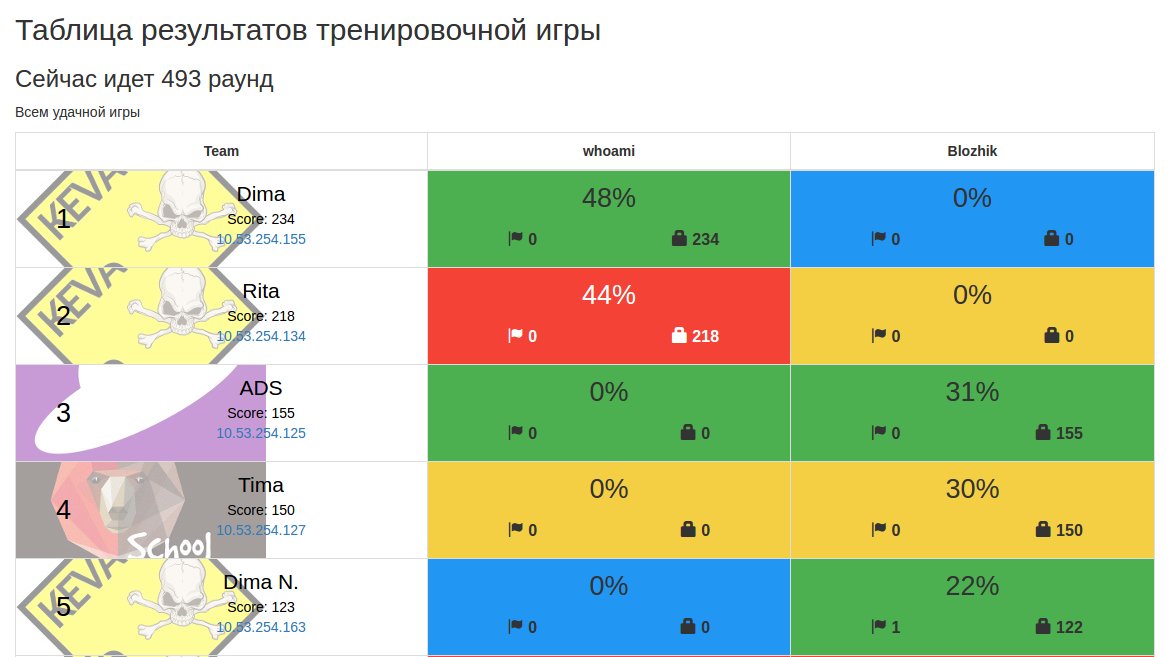
\includegraphics[width=0.75\linewidth]{images/scoreboard.png}}
\caption{Результат работы scoreboard.py}
\end{figure}

\begin{figure}[ht!]
Алгоритм работы модуля scoreboard представлен ниже (Рисунок 5.3).
\center{\includegraphics[width=0.25\linewidth]{individual_reports/score.png}}
\caption{Cхема работы scoreboard.py}
\end{figure}


\clearpage